% =========================== Main File =========================== %
%						  by Felix Strobel
%						    Licence: MIT
%			made for Munich University of Applied Sciences
%
% =========================== Main File =========================== %	



% =========================== Contribution =========================== %
% 					      Do you found a bug?
%				    Do you know a better solution?		
%					  You want to add a feature?
%
%				       Then follow these steps:
%    		Fork https://github.com/worldpotato/HM-LaTeX_Template
%						  Make your changes
%				   Create a well described Pull Request		
% =========================== Contribution =========================== %




% Document class
\documentclass[
	a4paper,
	12pt]
	{scrreprt}

% Packages
\usepackage[
	left= 2.5cm,
	right = 2cm, 
	bottom = 4 cm]
	{geometry}
% ============= Packages =============

% Documentinformations
% Hyperlink creations and PDF Informations
\usepackage[
	draft=true,
	pdftitle={title},
	pdfsubject={},
	pdfauthor={Your name},
	pdfkeywords={},
	pdfcreator={pdflatex},	
	%Links nicht einrahmen
	hidelinks
]{hyperref}


% Standard Packages
\usepackage[utf8]{inputenc}
\usepackage[english]{babel}
\usepackage[T1]{fontenc}
\usepackage{graphicx, subfig}
\usepackage{fancyhdr}
\usepackage{lmodern}
\usepackage{color}
\usepackage{transparent}
\usepackage{siunitx}

% for better lists
\usepackage{enumitem}

% additional characters of the American Mathematical Societey
\usepackage{amsfonts}
\usepackage{amsmath}

% for better looking paragraphs
% more infos at: http://www.khirevich.com/latex/microtype/
\usepackage[
	activate={true,nocompatibility}, % activate={true,nocompatibility} - activate protrusion and expansion
	final, % final - enable microtype; use "draft" to disable
	tracking=true, % tracking=true, kerning=true, spacing=true - activate these techniques 
	kerning=true, 
	spacing=true, 
	factor=1100, % factor=1100 - add 10% to the protrusion amount (default is 1000)
	stretch=10, % stretch=10, shrink=10 - reduce stretchability/shrinkability (default is 20/20)
	shrink=10]
	{microtype}


% infos about the document like author	
% =========================== Document Infos =========================== %
%		        Change the values befor you start writing
% =========================== Document Infos =========================== %
% Author
\newcommand{\myAuthor}{Felix Strobel}
\newcommand{\myTitle}{Zusammenfassung \\
Multisensornavigation}
\newcommand{\myDepartment}{Fakultät für Geoinformatik}
\newcommand{\myUniversity}{Hochschule für Angewandte Wissenschaften München}
\newcommand{\myThesisType}{Zusammenfassung}
\newcommand{\myDegree}{Bachelor of Engineering}
\newcommand{\myBirthDate}{01 January 1970}
\newcommand{\myBirthTown}{Musterhausen}
\newcommand{\myDocumentDate}{Juli 2019}
\newcommand{\myFirstExaminer}{Prof. Dr. med. Dr.-Ing. M. Mustermann}
\newcommand{\mySecondExaminer}{Prof. Dr.-Ing. F. Musterfrau}

	

\graphicspath{{img/}}

% Do not indent after paragraph
\setlength{\parindent}{0pt}

% additional hyphenation
\hyphenation{
	De-zi-mal-tren-nung
	}



% ============= Begin of document =============

\begin{document}


% Pages without header and footer
\pagestyle{empty}

	% =========================== Title Page =========================== %
%				       Don't change this file! 
%   			Change the values in /preable/documentInfos
% =========================== Title Page =========================== %

\begin{center}
\begin{tabular}{p{\textwidth}}

\begin{center}
	\def\svgwidth{200pt}
	\input{img/Hochschule_Muenchen_logo.pdf_tex}
\end{center}

\begin{center}
\LARGE{\textsc{
	\myTitle\\
}}
\end{center}

\\

\begin{center}	
	\large{\myDepartment \\
			of \myUniversity \\}
\end{center}

\\

\begin{center}
	\textbf{\Large{\myThesisType}}
\end{center}

\begin{center}
	geschrieben bei
\end{center}

\begin{center}
	\large{\textbf{\myAuthor}} \\
\end{center}

\begin{center}
\large{\myDocumentDate}
\end{center}

\\
\\

\end{tabular}
\end{center}

	% Ends a page and force printing all defined but not printed floating objects on all following pages. If neccessary a 	black page will be inserted to make sure that the next page has an odd number.
	\cleardoubleoddpage

% activate pagestyle for whole document
\pagestyle{fancy}
	% FancyHeader docu: http://mirrors.rit.edu/CTAN/macros/latex/contrib/fancyhdr/fancyhdr.pdf
% E: Even page
% O: Odd page
% L: Left field
% C: Center field
% R: Right field \slshape

\fancyhead[R]{\leftmark \slshape
\renewcommand{\headrulewidth}{0.4pt}}

	% FancyHeader docu: http://mirrors.rit.edu/CTAN/macros/latex/contrib/fancyhdr/fancyhdr.pdf
% E: Even page
% O: Odd page
% L: Left field
% C: Center field
% R: Right field

\fancyfoot[C]{\thepage}
\renewcommand{\footrulewidth}{0.0pt}
	
	\tableofcontents
	\setcounter{tocdepth}{1} % Show sections
	%\setcounter{tocdepth}{2} % + subsections
	

	% Index of pictures
	\listoffigures

	% Index of tables
	\listoftables


	
	
	%
\section{Kalmanfilter}
\label{sec:faq:kalmanfilter}


\subsection{Forward/Backward Algorithmus}
Die Nutzung der Varianzen, gerechnet vor vorne und hinten.
\subsection{Singulärwertzerlegung}
 Aufteilung in 3 Teilmatrizen. A = UDVt. U: eine unitäre  m x m-Matrix ist, D: Diagonalmatrix V:  die Adjungierte einer unitären n x n  n x n-Matrix V
\subsection{UWB Messungen, wie kann eine Trojektorie eschätzt werden}
Polynome vom Grad x (p(t) = a0 + a1t + a2t$^2$...) a0 + a1 * 0 + a2 * 0$^2$ + ... = [x0 y0]. Das ganze wird in Matrix-Vektor form gebracht.  Werte in der Struckturmatrix werden werden durch tn geteilt, um sie zu normalisieren. Anschließend in matlab mit ax = linsolve(A, ax)... 
\subsection{Was ist ein homogenes linieares Gleichungssystem}
Homogen: Auf den Nullraum abgebildet. (Rechter und untererer Rand sind 0). Lineares Gleichungssystem: gleich viel gleichungen wie unbekannte.
\subsection{Was ist ein überbestimmtes und inhomogenes gleichungssystem}
Ich bilde nicht auf dne Nullraum ab und habe mehr gleichungen als Unbekannte.

\subsection{Kernidee Integrity Monitoring}

Abweichungen von über 3 Sigma sind nicht zu verwenden.

\subsection{Phasen des Kalmanfilters}
\begin{description}
\item[Prediction Phase] Der Teil beim Kalmanfilter der als erstes ausgeführt wird, es wird das Bewegungsmodel verwendet und geschätzt wo wir sind.
\item[measurement update] die neue Messung kommt rein.
\item[Estimation] eigentlicher Filterschritt.
\end{description}

\subsection{wie lauten die Modellannahmen des Kalman Filters}
Normalverteilte Rauschen, Normalverteilt, Lineares Bewegungsmodel,
\subsection{Warum linear Verteilt}
Damit eine Normalverteilung normal bleibt. 

\subsection{warum ist die Modellannahme "linear" beim EKF wichtig?}

Dieser Arbeitet mit nicht linearen Modellen, welche linearisiert werden müssen.

\subsection{Warum Normalverteilungen}
Weil diese deutlich einfacher zu verarbeiten sind.  

\subsection{Was bewirkt der Kalmanfilter}
Verrechnet eine Schätzung aus einem Bewegungsmodell und der aktuellen Messung miteinander und schätzt dadurch den realen Wert.

\subsection{Warum ergibt eine neue Zustandsschätzung wieder eine Normalverteilung}

Weil wir nur Normalverteilungen haben und eine Normalverteilung * Normalverteilung = Normalverteilung
\subsection{Wenn Mittelwert bekannt, wie berechnung der Varian}
In Strucktur der Normalverteilung bringen und dann Varianz ablesen.
\subsection{Cartesian Motion}





\section{Kapitel 5}
\label{sec:faq:kap5}

\newpage

\chapter{Partikelfilter}
\label{kap6Partikelfilter}


	
	\section{WDF}
	Wahrscheinlichkeitsdichtefunktion \cite{wdf}
	
	\section{Mutation}
	Das verändern eines Messwertes von einer Generation zur nächsten
	
	\section{Modellannahmen des Partikelfilters}
	
	\begin{itemize}
		\item Sensoren nicht normalverteilt
		\item WDF kann multimodal / mit mehreren Peaks sein, damit kann ich mich Global positionieren
	\end{itemize}
	

		
	
	\section{Kalmanfilter vs. Partikelfilter}	
		\begin{itemize}
		\item Normalverteilt vs. nicht normalverteilt
		\item Linear vs. nicht linear
		\item Kalmanfilter ist mathematisch, Partikelfilter ist algorithmisch
	\end{itemize}

	\section{Generation}
		Eine Menge von N posen (Partikel) zum Zeitpunkt $X_k$ \\
		Jede Generation approzimiert die Wahrscheinlichkeitsdichtefunktion (WDF) anhand des momentan verfügbaren Wissens

	\section{Partikel}
		Eine Pose der Generation $X_k$
		
	\section{Schritte des Partikelfilter}

		Es gibt einen Init und fünf reguläre Schritte dazu noch einen um die Position zu berechnen
		
		\subsection{Init}
		Initialisierung durch Gleichverteilung von Partikeln
		
		\subsection{Bewegung}
		Bewegen des Roboters \textit{(Zeitpunkt k - 1)}
		
		\subsection{Messung}
		Messung durchführen \textit{(Zeitpunkt k)}
		
		\subsection{Propagation}
		Propagation aller Partikel durch Bewegungsmodell (Zeitpunkt k) (Mutation kann auch hier durchgeführt werden)
		Hier werden die Partikel mit dem Bewegungsmodel bewegt. \\
		Wenn $Q$ (Rauschen) mit 0 angenommen wird, \\
		$Q$ wird verwendet um das Rauschen der Sensoren zu imitieren. Außerdem wird es verwendet um die Partikel zu verteilen.
		
		\subsection{Gewichtung}
		Bewertung der Messungen für jedes Partikel. \\
		\\
		\textbf{Gewichtung Beispiel:} \\
		Differenz zwischen Partikelmessung und realer Messung. Reale Messung als Zentrum einer Normalverteilung und Gewichtung entspricht der Wahrscheinlichkeit in dieser Normalverteilung.
		
		\subsection{Neuverteilung der Partikel}
		Neuverteilung der Partikel mit Mutation
		
		\subsection{Berechnung der Position}	
		Berechnung der Position mittels gewichtetem Mittel oder ransac \cite{ransac} (\ref{uebersicht:sec:RANSAC})

	
	\section{Anzahl Schleifen in Init}
	Wieviel Schleifen in init


	\chapter{Stoffübersicht}
\label{chp:stoffübersicht}

\section{Homogene Matrix}	
\label{chp:stoffübersicht:sec:homogeneMatrix}
Matrix, die Positionen und Orientierung beinhaltet 
\begin{equation}
M = 
\left(
\begin{array}{cc}
R & T\\
0 & 1
\end{array}
\right)
=
\left(
\begin{array}{cccc}
r_{11} & r_{12} & r_{13} & t_{1} \\
r_{21} & r_{22} & r_{23} & t_{1} \\
r_{31} & r_{23} & r_{33} & t_{1} \\
0 	   & 0    & 0    & 1  
\end{array}
\right)	
\end{equation}

Wird verwendet, damit man einfacher rechnen kann.

\section{Pose}	
\label{chp:stoffübersicht:sec:pose}
Beschreibt die Lage eines Körpers. Mit seinen Raumkoordinaten und dem Heading im Bezug auf ein Referenzkoordinatensystem. \\
Im $R_2$ z.B.: $(x, y, \alpha)$

\section{Singulärwertzerlegung}	
\label{chp:stoffübersicht:sec:singulärwertzerlegung}
Zerlegung einer Matrix in 3 Spezielle Matrizen welche miteinander Multipliziert die grundlegende Matrix ergeben. Auf der Hauptdiagonalen der mittleren Matrix stehen die Singularitäten der grundlegenden Matrix. 

\section{Levenberg‐Marquardt}
\label{chp:stoffübersicht:sec:Levenberg‐Marquardt}
Der Levenberg-Marquardt-Algorithmus ist ein numerischer Optimierungsalgorithmus zur Lösung nichtlinearer Ausgleichs-Probleme mit
Hilfe der Methode der kleinsten Quadrate. Das Verfahren kombiniert das Gauß-Newton-Verfahren mit einer Regularisierungstechnik, die
absteigende Funktionswerte erzwingt. Deutlich robuster als das Gauß-Newton-Verfahren, das heißt, er konvergiert mit einer hohen
Wahrscheinlichkeit auch bei schlechten Startbedingungen, allerdings ist auch hier Konvergenz nicht garantiert. Ferner ist er bei
Anfangswerten, die nahe dem Minimum liegen, oft etwas langsamer. 

\section{Bündelblockausgleichung}
\label{chp:stoffübersicht:sec:Bündelblockausgleichung}
Das Optimieren der "Sehstrahlenbündel" einer 3D-Szene, die von mehreren Kameras bzw. von einer Kamera aus mehreren Perspektiven
aufgenommen wird. Bei der Bündelblockausgleichung können gleichzeitig die Positionen der Punkte im 3D-Raum, die Positionen und
Orientierungen der beobachtenden Kameras sowie deren interne Kalibrierparameter derart an die Messbilder angepasst werden, dass
verbleibende Fehler (z. B. Bildverzerrungen, Messfehler der Auswertung) möglichst optimal auf alle Beobachtungen verteilt werden.
Speziell wird der Begriff verwendet, um nicht nur einzelne Bildpaare (je 2 überdeckende Messbilder) photogrammetrisch auszuwerten,
sondern eine beliebige Anzahl von zusammenhängenden Bildern (Block) miteinander zu verknüpfen. Zur Berechnung könnte man z.B.
Levenberg-Marquardt-Algorithmus nehmen. 

\section{Trajektorie}
\label{chp:stoffübersicht:sec:Trajektorie}
Der Weg eines Objektes in abhänigkeit von der Zeit.\\
Stellt auch die Lösungskurve einer Differenzialgleichung dar.

\begin{equation}
P_{(t)} = 
\left(
	\begin{array}{c}
	a_0 + a_1t + a_2t^2 \\
	b_0 + b_1t + b_1t^2
	\end{array} 
\right)
\end{equation} 

\section{Koppelnavigation}
\label{chp:stoffübersicht:sec:Koppelnavigation}
Koppelnavigation oder dead reckoning ist das aneinanderfügen vergangener Standortmessungen, welche jeweils relativ zum letzten Messzeitpunkt sind.

\section{Sigma Point Kalman Filter}
\label{chp:stoffübersicht:sec:SigmaPointKalmanFilter}
Kalman Filter für nicht lineare Gleichungssysteme. Legt eine Normalverteilte Punktwolke um den aktuellen Punkt. Stabiler als der Kalmanfilter.\\
Er ist für sehr nicht lineare Zusammenhänge besser geeignet, da keine Linearisierung stattfindet.\\
Sowohl das Bewegungsmodell, wie auch das Messmodell können mit Sigmapoints berechnet werden. Es kann aber auch nur  das Messmodell mit Sigmapoints in den neuen Zustand überführt werden.

\section{Extended Kalman Filter}
\label{chp:stoffübersicht:sec:ExtendedKalmanFilter}
Der EKF ist eine nicht lineare Version des Kalman Filters welcher mittels einer Schätzung des 
aktuellen Mittels und der Covarianzen linearisiert wird. Diese Linearisierung kann zu einer Ungenauigkeit des Filters führen. In extremen Fällen kann es zu einer Divergenz des Filters führen. Der Filter erreicht eine First-Order accuracy \cite{order-accuracy}.

\section{ICP oder Scanmatching}
\label{chp:stoffübersicht:sec:ICPoderScanmatching}
\textbf{Iterative Closest Point} um den kürzesten Abstand zwischen zwei Punktwolken zu bestimmen. Wird genutzt um zwei verschiedene Punktwolken aufeinander anzupassen, dazu müssen diese bereits näherungsweise angepasst sein.

\section{Partikelfilter}
\label{chp:stoffübersicht:sec:Partikelfilter}
Kann aus dem Vergleich vieler Messungen zu einer bekannten "Karte" den Ort absolut bestimmen. Damit kann er sich global positionieren. Er benötigt deutlich mehr Speicher als der Kalmanfilter und ist etwas ineffizienter, aber durch die Möglichkeit der globalen Positionierung und des fehlen einer Linearisierung ist er stabiler als ein Kalmanfilter.

\section{RANSAC}
\label{chp:stoffübersicht:sec:RANSAC}
Random sample consensus - Eine iterative Methode um outliner zu erkennen oder eine Gerade durch eine Punktwolke zu legen, welche viele outliner hat. Er wird u.A. im Bereich des Maschinellen Sehens verwendet um eine um Ausreißer bereinigte Datenmenge (Consensus Sets) zu erstellen. Das Consensus Sets findet in Verfahren, welche die Methode der kleinsten Quadrate verwendet, besonders wichtig, da diese mit Zunahme der Ausreißer instabiler werden.

\section{Loop closure}
\label{chp:stoffübersicht:sec:LoopClosure}
Wenn Messungen einen geschlossenen loop bilden. Dies kann genutzt werden um Filter und Ausgleichungen zu testen oder zu verbessern.

\section{SLAM}
\label{chp:stoffübersicht:sec:SLAM}
\textbf{Simultaneous localization and mapping} - Zeitgleiches Positionieren und Mapping der Messdaten. Wird in unbekannter Umgebung verwendet um eine Map zu erstellen in der sich dann positioniert werden kann.


	\chapter{Einführung}
\label{chp:einfuehrung}	

\section{Lokalisieren}
\label{chp:einfuehrung:sec:lokalisieren}
Die Fähigkeit sich gegenüber eines Bezugssystem zu Positionieren.
	
\section{3D Konstruieren}
\label{chp:einfuehrung:sec:3DKonstruieren}
Daten werden immer vom aktuellen Standort aus aufgenommen. Diese können dann nach einer Lokalisierung ins Globale System überführt werden.\\
Wenn Daten von mehreren Positionen aus aufgenommen werden, so muss die Position der Sensoren zueinander bekannt sein.

\section{Mobile Mapping System}
\label{chp:einfuehrung:sec:MobileMappingSystem}

Eigenschaften eines Mobile Mapping Systems:
\begin{enumerate}
	\item Mobile Plattform (Roboter, Flugzeug, Auto, etc.)
	\item Multisensoraufbau zur Vermussung der Umgebung in zwei- oder dreidimensionaler Form
	\item Berechnung des Umgebungsmodels online aber auf offline möglich.
\end{enumerate}

	\chapter{Mathematische Grundlagen}
\label{chp:MathematischeGrundlagen}




\section{Skalarprodukt}
\label{chp:MathematischeGrundlagen:sec:skalarprodukt}

	\begin{equation}
		\vec{a} \circ \vec{b} = |\vec{a}| \cdot |\vec{b}| \cdot \cos\varphi 
	\end{equation}
	\begin{equation}
		\vec{a} \circ \vec{b} =
		\left(
		\begin{array}{c}
		a_{x} \\
		a_{y}
		\end{array}
		\right) 
		\cdot 
		\left(
		\begin{array}{c}
		b_{x} \\
		b_{y}
		\end{array}
		\right)
		=
		a_{x}b_{x}
		+
		a_{y}b_{y} 
	\end{equation}

\section{Winkel zwischen zwei Vektoren}
\label{chp:MathematischeGrundlagen:sec:winkelVektoren}
	\begin{equation}
		\cos\varphi = \frac{\vec{a} \circ \vec{b}}{|\vec{a}| \cdot |\vec{b}|}
	\end{equation}	


\section{Orthogonalität}
\label{chp:MathematischeGrundlagen:sec:Orthogonalität}
	Zwei Vektoren $\vec{a}$ und $\vec{b}$ sind Orthogonal zueinander wenn das Vektorprodukt 0 ergibt.
		\begin{equation}
			\vec{a} \circ \vec{b} = 0
		\end{equation}

\section{Vektorprodukt}
\label{chp:MathematischeGrundlagen:sec:Vektorprodukt}
	\begin{equation}
		\vec{a} \times \vec{b} = \vec{c}
	\end{equation}
	\begin{equation}
		|\vec{c}| = |\vec{a}| \cdot |\vec{b}| \cdot \sin\varphi 
		\quad \textrm{for} \quad 
		(\ang{0} \leq \varphi \leq \ang{180})
	\end{equation}

\subsection{Matrix/Vektorform}

\begin{equation}
\vec{a} \times \vec{b} = 
\left(
\begin{array}{c}
a_{x} \\
a_{y} \\
a_{z}
\end{array}
\right)
\times
\left(
\begin{array}{c}
b_{x} \\
b_{y} \\
b_{z}				
\end{array}
\right)
= 
\left(
\begin{array}{c}
a_{y}b_{z} - b_{z}a_{y} \\
a_{z}b_{x} - b_{x}a_{z} \\
a_{x}b_{y} - b_{y}a_{x}  
\end{array}
\right)				
\end{equation}

\section{Rechte Hand Regel}
\label{chp:MathematischeGrundlagen:sec:RechteHandRegel}
	Die Rechte Hand gibt die Richtung der Achsen vor, die Vektoren (Finger) bilden ein Rechtssystem deren Vektorprodukte alle 0 ergeben.
	\begin{itemize}
		\item Daumen: X
		\item Zeigefinger: Y
		\item Mittelfinger: Z
	\end{itemize}


\section{Rotation}
\label{chp:MathematischeGrundlagen:sec:Rotation}

\subsection{Definition}
\begin{enumerate}
	\item Winkel der Drehung um jeweils eine Achse
	\item Rotationsmatrix multipliziert mit der Transponierten ergibt die Einheitsmatrix $I$
	\item Spalten stehen Senkrecht aufeinander
\end{enumerate}

\subsection{Rotation vs. Spiegelung}

	\subsection{Rotation}
 		Überführt ein Rechtwinkliges/Rechtshändiges Koordinatensystem in ein anderes Rechtwinkliges/Rechtshändiges Kooridinatensystem. RxR ist Einheitsmatrix.
 	\subsection{Spiegelung}
		Die Hand wechselt. Die Detimernante wird -1

\subsection{Prüfung auf Rotation}

\begin{lstlisting}[
style      = Matlab-editor,
basicstyle = \mlttfamily,
]
if abs(max(max((rotation * rotation') - eye(3)))) > 0.0000000000001
isRotation = false;
else
isRotation = true;

\end{lstlisting}


\section{Homogene Matrix}
\label{chp:MathematischeGrundlagen:sec:HomogeneMatrix}

Eine Homogene Matrix kann als Koordinatensystem interpretiert werden und stellt die Rotation sowie Translation des Systems in Bezug zu einem Anderen dar.

\subsection{Translation und Rotation}
\begin{equation}
	M = 
	\left(
	\begin{array}{cc}
		R & T\\
		0 & 1
	\end{array}
	\right)
	=
	\left(
	\begin{array}{cccc}
		r_{11} & r_{12} & r_{13} & t_{1} \\
		r_{21} & r_{22} & r_{23} & t_{2} \\
		r_{31} & r_{32} & r_{33} & t_{3} \\
		0 	   & 0    & 0    & 1  
	\end{array}
	\right)	
\end{equation}

\subsection{Vorteile}
	Mehrere Bewegungen können durch Matrixmultiplikation aneinander gekettet werden bzw. leichter invertiert werden.

\subsection{Intepretation als Koordinatensystem}

Eine Homogene Matrix kann auch als Koordinatensystem interpretiert werden. 



\subsection{Berechnung Koordinatenursprung}

\begin{equation}
T
=
\left(
\begin{array}{c}
t_{1} \\
t_{2} \\
t_{3} \\
\end{array}
\right)	
\end{equation}


\subsection{Berechnung der Achsen}
\begin{equation}
x =
\left(
\begin{array}{c}
r_{11}  \\
r_{21} \\
r_{31} \\
\end{array}
\right),	
y =
\left(
\begin{array}{c}
r_{12}  \\
r_{22} \\
r_{32} \\
\end{array}
\right),	
z =
\left(
\begin{array}{c}
r_{13}  \\
r_{23} \\
r_{33} \\
\end{array}
\right)	
\end{equation}


\section{Koordinatensysteme}
\label{chp:MathematischeGrundlagen:sec:Koordinatensysteme}

\subsection{Affines Koordinatensystem}
Lineare Koordinatensystem

\subsection{Orthogonales Koordinatensytem}
Rechtwinklig

\subsection{Orientierungstreues Koordinatensystem}
Es bleibt nach der rechten Hand definiert.

\section{RPY Darstellung}
\label{chp:MathematischeGrundlagen:sec:RPY}
Jede Rotation kann als Roll, Pitch, Yaw dargestellt werden.

\begin{tabular}{cc}
	Roll & X-Achse \\
	Pitch & Y-Achse \\
	Yaw & Z-Achse
\end{tabular}


\subsection{Rotation als RPY}
Dabei können Singularitäten auftreten. (Bei Pitch = $\pi/2 $ bzw. 90\textdegree) \\
	\textbf{Matrix to RPY}
\begin{lstlisting}[
style      = Matlab-editor,
basicstyle = \mlttfamily,
]
y = atan2(rotation(2,1), rotation(1,1));
p = atan2(-rotation(3,1), rotation(1,1) * cos(y) + rotation(2,1) * sin(y));
r = atan2(rotation(3,2)/cos(p), rotation(3,3)/cos(p));
\end{lstlisting} 

\subsection{RPY to Matrix}
Eine Rotation, welche zuerst um die Roll, dann die Pitch und zuletzt die Yaw achse dreht

\begin{equation}
R_{\alpha, \beta, \gamma} % rpy
=
\left(
\begin{array}{ccc}
\cos{\alpha}\cos{\beta} & \cos{\alpha}\sin{\beta}\sin{\gamma} - \sin{\alpha}\cos{\gamma}  & \cos{\alpha}\sin{\beta}\cos{\gamma} + \sin{\alpha}\cos{\gamma} \\
\sin{\alpha}\cos{\beta} & \sin{\alpha}\sin{\beta}\sin{\gamma} + \cos{\alpha}\cos{\gamma} & \sin{\alpha}\sin{\beta}\cos{\gamma} - \cos{\alpha}\sin{\gamma}  \\
-\sin{\beta}	   & \cos{\beta}\sin{\gamma}    &   \cos{\beta}\cos{\gamma}
\end{array}
\right)	
\end{equation}


\subsection{Weitere Darstellungen}
\begin{itemize}
	\item Quaternionen \cite{quaternionen}
	\item Axis/Angle Darstellung \cite{axis-angle} -> numerisch stabil
\end{itemize}


	\chapter{Cartesian Motion}
\label{chp:cartesianMotion}
Cartesian Motion ist eine Bewegung auf $n$ rechtwinklig zueinander stehenden Achsen.

\section{Glatter Übergang zwischen zwei Koordinatensystemen}
Um den Übergang zwischen Koordinatensystemen zu berechnen muss für die Rotation die RPY Darstellung [\ref{chp:MathematischeGrundlagen:sec:RPY}] verwendet werden. \\
Anschließend wird Komponentenweise interpoliert.


\begin{enumerate}
\item Interpolieren von RPY
\begin{equation}
		\begin{array}{l}
		r^{(i)}(s) := (1 - s) \cdot r^{(0)} + sr^{(N)}
 \\
		p^{(i)}(s) := (1 - s) \cdot p^{(0)} + sp^{(N)}
\\
		y^{(i)}(s) := (1 - s) \cdot y^{(0)} + sy^{(N)}
\\
		\\
		mit \; s := \frac{k}{N+1} \;|\; k \; \in \{1,...,N-1\}
		
		
		\end{array}
\end{equation}

\item Interpolieren des Ursprungs

\begin{equation}
\begin{array}{l}
T_x^{(i)}(s) := (1 - s) \cdot T_x^{(0)} + sT_x^{(N)}
\\
T_y^{(i)}(s) := (1 - s) \cdot T_y^{(0)} + sT_y^{(N)}
\\
T_z^{(i)}(s) := (1 - s) \cdot T_z^{(0)} + sT_z^{(N)} \\
\end{array}
\end{equation} 	
\end{enumerate}


\section{Warum nicht mit 3x3 Matrix}
Da die Eigenschaften der Drehungen verloren gehen würden. Daher:

\begin{enumerate}
	\item Überführung in RPY Darstellung
	\item Überführung in nächstes Koordinatensystem.
	\item Zurück in Rotationsmatrix
\end{enumerate}

\section{Nachteil von RPY Darstellung}
Dabei können Singularitäten auftreten. Bei Pitch = $\pi/2 $ bzw. 90\textdegree) \\

	\chapter{Trajektorie}
\label{chp:trajektorie}

\section{Definition}
Der Weg eines Objektes in Abhängigkeit von der Zeit.\\
Stellt auch die Lösungskurve einer Differenzialgleichung dar.

\begin{equation}
P_{(t)} = 
\left(
\begin{array}{c}
a_0 + a_1t + a_2t^2 \\
b_0 + b_1t + b_1t^2
\end{array} 
\right)
\end{equation} 

\section{Quintisches Polynom}
Ein Quintisches Polynom enthält 6 Komponenten $\{a_0, a_1, a_2 , ..., a_5\}$ und ist, wie der Name vermuten lässt, vom 5. Grad. \\

\subsection{Interpolations Annahmen}
Es werden $Freiheitsgrad + 1$ Annahmen benötigt. \\
Diese können z.B. Position, Geschwindigkeit und Beschleunigung jeweils für den Start- und End-Punkt.\\
\\
Alternativ könnten auch Position, Range und Bearing jeweils für den Start und End-Punkt als Annahme dienen.

\subsection{Pseudocode Implementierung}
\begin{enumerate}
	\item Erstellen der Strukturmatrix mit Normierter Zeit variable  $A$(1x6)
	\item Erstellen des Ergebnisvektors $b$ (2x1)
	\item Lineares Gleichungssystem lösen
	\item Zeitpunkt bestimmen, an dem die Position bestimmt werden soll.
	\item Zeitpunkt in Gleichungssystem einsetzen
\end{enumerate}

\subsection{Überbestimmung}
Wenn es mehr Interpolationsbedingungen als Freiheitsgrade gibt ist es nicht mehr eindeutig zu lösen. Dies führt zu einer Unsicherheit.

\subsection{Vorteile des Quintischen Polynoms}
\begin{itemize}
	\item Beschreiben der Trajektorie speicherarm als Mathematische Funktion.
	\item Einfaches Interpolieren
\end{itemize}

\subsection{Vorteile von Endpunkt $T = 1$}
Das Polynom bleibt dadurch numerisch stabiler.


	\chapter{Kalmanfilter}
\label{chp:kalmanfilter}

\section{Eigenschaften}
\begin{enumerate}
	\item Asymptotisch stabil
	\item Kein anderer Schätzer liefert Schätzwerte mit kleinerer Varianz
	\item Schätzwerte sind erwartungstreu (unbiased)
	\item Ohne Rauschen ist er identisch zu einem rekursiven LSQ-Schätzer \footnote{LSQ = 	Least Squares Quadratic}
	\item Er liefert den wahrscheinlichsten Schätzwert 
\end{enumerate}

\section{Modellannahmen des Kalmanfilters}
\begin{itemize}
	\item Rauschen ist zufällig - normalverteilt und nicht systematisch
	\item Lineare Abbildung, damit die Normalverteilung eine Normalverteilung bleibt.
	\item Das Rauschen ist Zufällig.
\end{itemize}

Die Abbildung muss linear sein, damit die Varianz-Kovarianz Matrix im Anschluss immer noch eine Normalverteilung darstellt. (Die Normalverteilung muss eine Normalverteilung bleiben).

\section{Anwendung und Wirkweise}
Der Kalmanfilter wird verwendet um mittels einer Messung einen neuen Schätzwert zu bestimmen. Dies geschieht mit Hilfe des gewichteten Mittels.

\section{Erweiterter Kalmanfilter}
Der Kalmanfilter Arbeitet mit einem nicht linearen Zusammenhang. Allerdings wird dieser Zusammenhang mittels der Taylorapproximation \footnote{Partielle Ableitung} linearisiert, sodass die Normalverteilung bestehen bleibt.

\section{Vorteile der Normalverteilung}
\begin{itemize}
	\item Normalverteilungen lassen sich einfach miteinander Verrechnen
	\item Das Messrauschen ist meist auch normalverteilt
\end{itemize}

\section{Extremwert/Mittelwert der Normalverteilung}
Der Mittelwert und Extremwert einer Normalverteilung sind identisch.

\section{Kernidee der Schätzung}
Die Kernidee hinter der Schätzung ist, dass sowohl das Messmodell wie Bewegungsmodell einen Fehler haben und die Wahrheit in der Mitte liegt. Um den Mittelwert der zwei Normalverteilungen zu berechnen werden sie zueinander auch noch gewichtet. 

\begin{figure}[!ht]
	
	\begin{center}                                      
		
		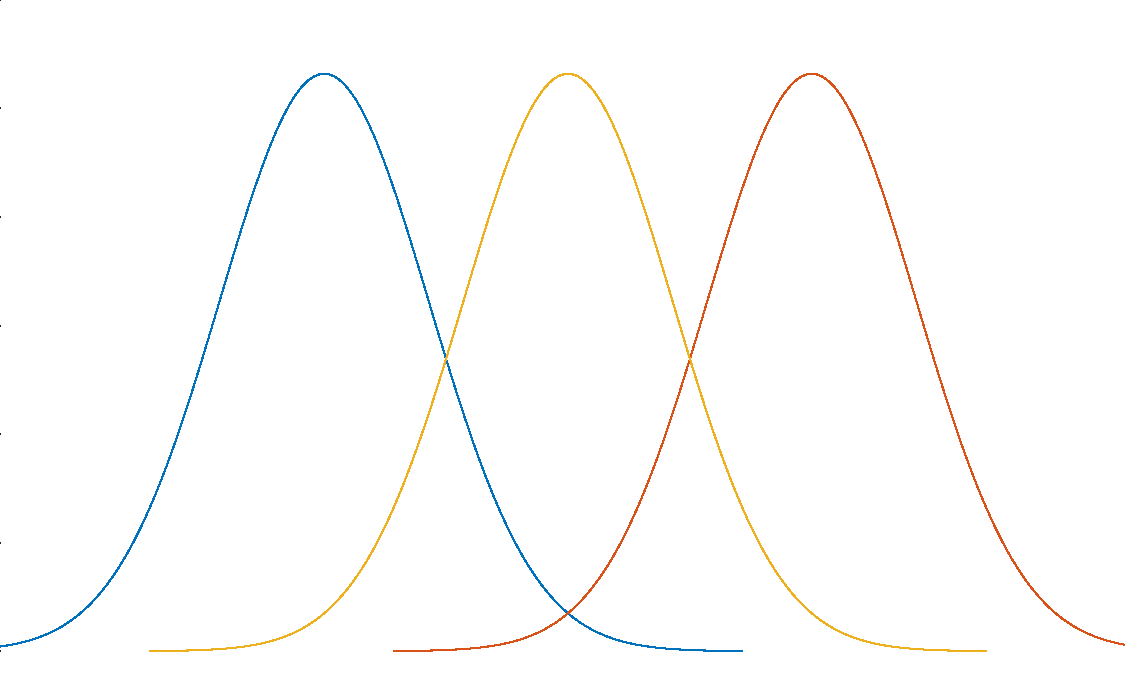
\includegraphics[width=0.7\textwidth, height=100px]{normal_distributions.pdf}                                                                  
		
	\end{center}
	\caption{Grundidee des Kalmanfilters}
	\label{fig:kernideeKalman}
	
\end{figure}

\section{Innovation}
Die Innovation des Kalmanfilters ist der Vergleich zwischen Messung und Schätzung des Kalmanfilters. 

\section{Parameter des Update Gain}
Die Standardabweichung der Messung so wie die der Schätzung.\\
Das Update Gain wird wie folgt berechnet: \~{}

\begin{equation}
K = \frac{(\bar{\sigma}_k)^2}{(\bar{\sigma}_k)^2 + (\tilde{\sigma}_k)^2}\\
\end{equation}

\section{Wertebereich des Update Gain}
Der Wertebereich des Gain ist normalisiert. $[0, 1]$ \\

\section{Eingrenzung des Mittelwertes einer Schätzung}

Der Mittelwert der \textbf{neuen Schätzung} $\hat{x}_k$ wird mittels des Gain $K$, der \textbf{vorherigen Schätzung} $\bar{x}_k$ und der \textbf{neuen Messung} $\tilde{x}_k$ berechnet.

\begin{equation}
\hat{x}_k = \bar{x}_k + K \left( \tilde{x}_k - \bar{x}_k \right) 
\end{equation}

\section{Berechnung der Varianz}
\begin{equation}
\hat{\sigma}^2_k = \left( 1 - K \right) (\bar{\sigma_k})^2
\end{equation}







	\chapter{Kalmanfilter Gleichungen}
\label{chp:kalmanfilterGleichungen}

\section{Begriffserklärungen}
\begin{description}
	\item[Predicition Phase] Schätzen des Zustandes als Normalverteilung mit dem Bewegungsmodell $F$ (z.B. aus Odometrie) und dem Bewegungsrauschen $Q$
	\item[Measurement update] Durchführung einer Messung $z$ als Normalverteilte Zufallsvariable mit Messrauschen $R$
	\item[Estimation] Berechnung des Kalman Gain $K$ aus geschätztem Zustand und neuer Messung mit Zustandsraummodellierung $H$. Daraus
	berechnet sich neuer Systemzustand $x$ und $P$
	\item[a priori state estimate] Der in Schritt 1 geschätzte Systemzustand \textit{NV}($\bar{x}_k, \bar{P}_k$). Dieser wird \underline{ohne} einer neuen Messung geschätzt.
	\item[a posteriori state estimate] Der in Schritt 3 geschätzte Systemzustand \textit{NV}($\hat{x}_k, \hat{P}_k$). Dieser wird \underline{mit} einer neuen Messung geschätzt.
\end{description}



\section{Gleichungen}

% In dem enumerate sind jeweils die Formeln mit der Legende als tabular
\begin{enumerate}
	\item \textbf{Prediction phase}
	\begin{equation}
	 \bar{x}_k = F \, \hat{x}_{k-1}
	\end{equation}
	
	\begin{tabular}{cl}
	$F$ &:= Bewegungsmodell \\
	$\hat{x}_{k-1}$ &:= Schätzung aus letztem Durchgang
	\end{tabular}
	
	\begin{equation}
	\bar{P}_k = F \, \hat{P}_{k-1} \, F^t + Q_{k-1}
	\end{equation}
	
	\begin{tabular}{cl}
	$\bar{P}_k$ & := a priori state estimate \\
	$\hat{P}_{k-1}$ & := a posteriori state estimate des vorherigen Durchgangs \\
	$Q_{k-1}$ & := Rauschen des vorherigen Durchgangs \\
	\end{tabular}
	
	
	
	
	\item \textbf{Measurement update}
	
	\begin{equation}
		\tilde{z}_k = Messung + \tilde{R}_k
	\end{equation}
	
	\begin{tabular}{cl}
		$\tilde{z}_k$ & := neue Messung \\
		$\tilde{R}_k$ & := Rauschen der Messung
	\end{tabular}
	
	
	

	\item \textbf{Estimation}
	
	\begin{equation}
	K_k = \frac{\bar{P}_k \, H^t_k} {(H_k \, \bar{P}_k \, H^t_k + \tilde{R}_k)}
	\end{equation}
	\begin{tabular}{cl}
		$K_k$ & := neuer Kalman Gain \\
		$H_k$ & := Messmodell
	\end{tabular}


	\begin{equation}
		\hat{x}_k = \bar{x}_k + K_k \, (\tilde{z}_k - H_k \, \bar{x}_k)
	\end{equation}
	In dieser Gleichung werden die zwei Normalverteilungen in eine neue überführt (vgl. \ref{fig:kernideeKalman}). 
	
	\begin{tabular}{cl}
		$H_k \, \bar{x}_k$ & := $\bar{z}_k$ und entspricht damit der Schätzung über das Messmodell\\
	\end{tabular}

	\begin{equation}
		\hat{P}_k = (I - K_k \, H_k)\bar{P}_k
	\end{equation}
	
\end{enumerate}

\section{Integrity Monitor}
Ein Integrity Monitor erkennt Außreiser und filtert diese. Beim Kalmanfilter bedeutet dies, dass die Messung nicht verwendet wird und dieser eine Schritt nur mit dem Bewegungsmodell geschätzt wird. \\
Typischerweise werden Messungen welche außerhalb von $ 3 \, \sigma $ liegen, als Ausreiser deklariert.

\section{Multisensorentwurf}
Um mehrere Sensoren mit unterschiedlichen Taktraten zu Fusionieren wird mit der höchsten verfügbaren Taktrate \footnote{Meist ist dies der Odometriesensor oder die IMU} durch eine Schleife iteriert. Innerhalb dieser Schleife wird jeder Sensor abgefragt ob gerade ein neuer Messwert vorhanden ist. //
Wenn ein neuer Messwert vorhanden ist, wird dieser Verwendet um eine neue Position zu schätzen und den posteriori zu aktualisieren. 
	\chapter{Range Bearing}
\label{chp:rangeBearing}

Range Bearing Sensoren werden in der Robotik häufig verwendet. Sie geben eine Entfernung und eine Richtung, bezogen auf das Heading, zu einem Messpunkt.

\section{Bewegungsmodell}
\label{chp:rangeBearing:sec:bewegungsmodell}

Auf die aktuelle Pose des Roboters wird die Veränderung addiert. Es wird ein rechtwinkliges Dreieck aufgespannt über das die
Veränderung beschrieben werden kann. Zur Linearisierung werden die Terme partiell abgeleitet zunächst nach $x$, $y$, Winkel (Jacobi Fx) und
dann nach dem Rauschen in Distanz $d$ und Winkel $\alpha$ (Jacobi Fv).

\section{Messmodell}
\label{chp:rangeBearing:sec:messmodell}
Zwischen einer Landmarke und der akutellen Position wird ein rechtwinkliges Dreieck aufgespannt auf dem die Hypothenuse der Distanz
zwischen Position und Landmarke entspricht. Die Orientierung entspricht dem Tangens der beiden Katheten in diesem Dreieck. Zur
Linearisierung werden die Terme partiell abgeleitet nach $x$, $y$, Winkel für das Messmodell $H_x$. Das Messrauchen (hier: $W$) wird außerhalb
des Modells addiert und ergibt nach Linearisierung eine Einheitsmatrix $H_w$
	\chapter{Singulärwertzerlegung}
\label{chp:singulaerwertzerlegung}
 Eine Singulärwertzerlegung ist die Aufteilung in 3 Teilmatrizen. 
 
 \begin{equation}
 	A = UDV^t
 \end{equation}
 
 \begin{tabular}{cl}
 	U & := eine unitäre  m x m-Matrix \\
 	D & := Diagonalmatrix mit Eignevalues \\
 	V & := Adjungierte einer unitären n x n Matrix
 \end{tabular}

\section{Pseudoinverse}

Eine Pseudoinverse bildet die auf sinuläre Matrizen verallgemeinerte Inverse einer Matrix.

\begin{equation}
A^t := VD^{-1}U^t \; mit \; diag(D^{-1}) = \frac{1}{\sigma})
\end{equation}

Dann heißt die so berechnete Matrix Pseudoinverse $A^t$. 

\section{Anwendung}

\subsection{Nichtsingulär}

Eine Matrix ist genau dann nichtsingulär, wenn 
\begin{equation}
\forall \sigma: \sigma = 0
\end{equation}


\subsection{Schlecht konditioniert}
Eine Matrix ist schlecht konditioniert, wenn

\begin{equation}
\frac{\sigma_{n-1}}{\sigma_0} \approx 0
\end{equation}

Dies hat zur Folge, dass der Gleichungsterm nicht stabil gelöst werden kann.
 

	
	% references
	\bibliographystyle{unsrtdin}
	\bibliography{bib/literature}

\end{document}
